\documentclass[conference]{IEEEtran}
\usepackage{amsmath,amssymb}
\usepackage{graphicx}
\usepackage{booktabs}
\usepackage{siunitx}
\usepackage{xcolor}
\usepackage[hidelinks]{hyperref}
\usepackage[capitalise]{cleveref}

% numbers generated from the measurements (speed_vlm/paper_figs.py, speed_vlm/baselines.py)
\newcommand{\TtftMin}{0.42}
\newcommand{\TtftMax}{11.1}
\newcommand{\TtftRatio}{26}
\newcommand{\VisShareMax}{96}
\newcommand{\TpotMs}{52}
\newcommand{\VstarMin}{0.39}
\newcommand{\VstarMax}{2.77}
\newcommand{\VstarRatio}{7}
\newcommand{\FitRtwo}{0.995}
\newcommand{\GpuSpMin}{2.4}
\newcommand{\GpuSpMax}{2.7}
\newcommand{\CpuEffect}{6}
\newcommand{\PActMin}{8.0}
\newcommand{\PActMax}{16.9}
\newcommand{\PIdleMin}{4.9}
\newcommand{\PIdleMax}{6.3}
\newcommand{\EreqBest}{14}
\newcommand{\GovGpu}{882}
\newcommand{\GovCpu}{1238}
\newcommand{\GovSlowMax}{47}
\newcommand{\NInputs}{36}
\newcommand{\NReq}{3960}

\newcommand{\NScen}{798}
\newcommand{\Dq}{2}
\newcommand{\OracleSaveCont}{39}
\newcommand{\OracleSaveEvent}{19}
\newcommand{\GovSaveCont}{12}
\newcommand{\GovSaveEvent}{8}
\newcommand{\GovViolCont}{8.4}
\newcommand{\GovViolEvent}{12.8}
\newcommand{\OracleVsGovCont}{30}
\newcommand{\OracleVsGovEvent}{12}
\newcommand{\SpeedOnlySaveCont}{21}
\newcommand{\InputOnlySaveCont}{20}
\newcommand{\RaceSaveCont}{15}
\newcommand{\RaceSaveEvent}{13}


\newcommand{\todo}[1]{\textcolor{red}{[TODO: #1]}}
\newcommand{\Lq}{L_{q}}
\newcommand{\nact}{n_{\mathrm{act}}}

\begin{document}
\title{Speed- and Input-Aware DVFS for On-Robot Vision-Language Models}
\author{\todo{authors}}
\maketitle

\begin{abstract}
\todo{abstract}
\end{abstract}

% =====================================================================================================
\section{Motivation}
\label{sec:motivation}

We run a vision-language model (VLM), Qwen2.5-VL-3B (Q4\_K\_M, llama.cpp), alone on a Jetson Orin NX 16\,GB
and measure every request in stages (image preprocessing, vision encoder, image prefill, text prefill,
decode). The workload matrix covers \NInputs{} inputs, i.e.\ four resolutions
(224$\times$168 to 672$\times$504) $\times$ 1/2/4 images $\times$ 32/128/512 text tokens, at
3 CPU $\times$ 7 GPU clocks plus the stock governors (\NReq{} requests in total).
The input is fixed by the task, the speed is fixed by the planner, and DVFS is the only knob.
We make four observations.

\paragraph{O1: The input sets the latency, over more than an order of magnitude}
At the highest clocks, the time-to-first-token (TTFT) ranges from \TtftMin\,s to \TtftMax\,s
(\TtftRatio$\times$) across inputs (\cref{fig:mot-input}a).
The vision path (encoder plus image prefill) accounts for up to \VisShareMax\% of TTFT, so the
number of visual tokens $N_{\mathrm{vis}}$, i.e.\ resolution times number of images, is the dominant
factor; text length is secondary.
Decoding costs about \TpotMs\,ms per token independently of the input, so the time until the robot
has the $\nact$ tokens it needs to act is $\mathrm{TTA}(\nact)\approx\mathrm{TTFT}+(\nact-1)\,\mathrm{TPOT}$.

\paragraph{O2: Speed turns latency into a hard constraint}
While the VLM computes, the robot keeps moving; once the answer is available it must still be able
to stop within the decision distance $D$:
\begin{equation}
  v\,(\Lq + t_{\mathrm{act}}) + \frac{v^2}{2a} + m \le D
  \;\Longleftrightarrow\;
  \Lq \le \tau(v) \triangleq \frac{D - m - v^2/2a}{v} - t_{\mathrm{act}},
  \label{eq:safety}
\end{equation}
where $\Lq$ is the $q$-quantile ($q{=}0.95$) of $\mathrm{TTA}(\nact)$, $a$ the braking deceleration,
$t_{\mathrm{act}}$ the actuation delay and $m$ a margin
($D{=}5$\,m, $a{=}2$\,m/s$^2$, $t_{\mathrm{act}}{=}0.05$\,s, $m{=}0.5$\,m).
Inverting \cref{eq:safety} gives the maximum safe speed $v^*$ an input supports. Even at the highest
clocks, $v^*$ ranges from \VstarMin\ to \VstarMax\,m/s (\VstarRatio$\times$) across inputs
(\cref{fig:mot-input}b). Speed and input are therefore coupled: the same speed requires very different
latencies, and hence clocks, for different inputs.

\paragraph{O3: The GPU clock is the only effective knob, and the two ways of counting energy disagree}
Latency follows $a + b/f_{\mathrm{GPU}}$ ($R^2 \ge \FitRtwo$), and raising the GPU clock from 306 to
918\,MHz shortens TTFT by \GpuSpMin--\GpuSpMax$\times$ (\cref{fig:mot-dvfs}a). The CPU clock changes
latency by at most $\pm$\CpuEffect\% but adds power, so it should stay low.
Active board power doubles across the clock range (\PActMin--\PActMax\,W), whereas idle power varies
only between \PIdleMin\ and \PIdleMax\,W (\cref{fig:mot-dvfs}b). As a consequence, the energy per request is
lowest at the \emph{highest} GPU clock with the lowest CPU clock (\EreqBest\% below max clocks,
\cref{fig:mot-dvfs}c), while the average power of a continuously running VLM is lowest at the
\emph{lowest} clocks. The best clock therefore depends on how the robot invokes the VLM.

\paragraph{O4: The stock governor is oblivious to both input and speed}
Under VLM load, the stock governors (schedutil and nvhost\_podgov) settle near
\GovGpu\,MHz GPU and \GovCpu\,MHz CPU regardless of the task. This wastes power at low speed, yet is
up to \GovSlowMax\% slower than the highest clocks and therefore misses deadlines at high speed
(\cref{sec:exp-results}). The clock an oracle would choose varies over the whole range across
(input, speed) pairs (\cref{fig:mot-oracle}), so no fixed setting, and no policy that sees only the
speed or only the input, is sufficient.

\begin{figure*}[t]
  \centering
  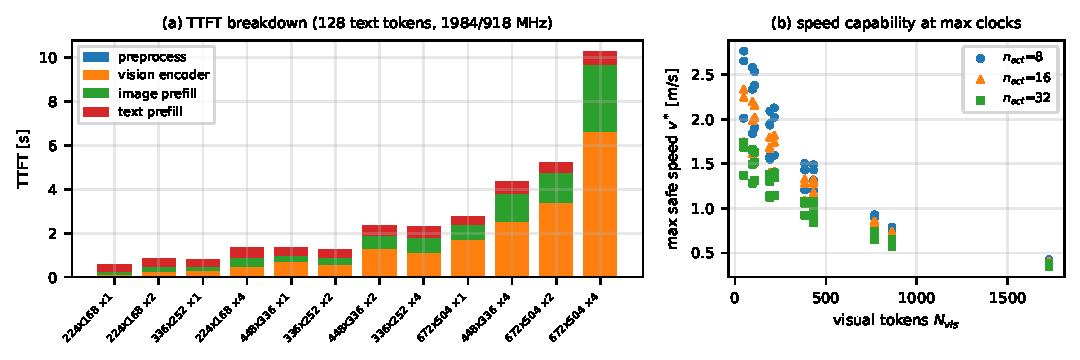
\includegraphics[width=\textwidth]{figs/mot_input_latency.pdf}
  \caption{(a) TTFT breakdown per input at 1984/918\,MHz; the vision path dominates.
  (b) Maximum safe speed $v^*$ (\cref{eq:safety}) at the highest clocks versus the number of visual tokens.}
  \label{fig:mot-input}
\end{figure*}

\begin{figure*}[t]
  \centering
  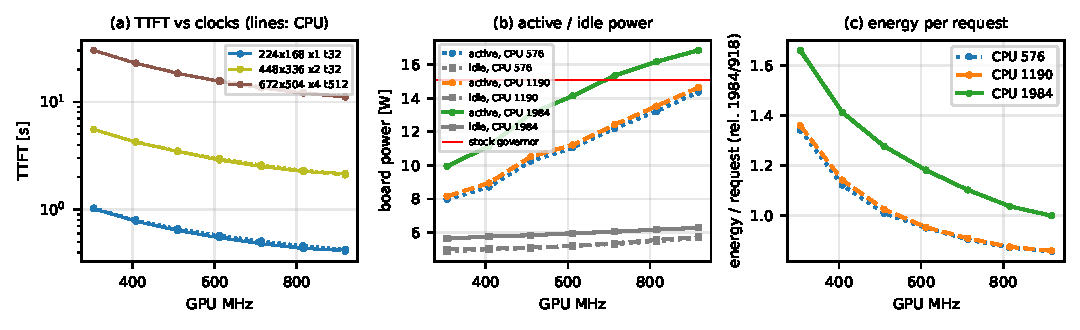
\includegraphics[width=\textwidth]{figs/mot_dvfs.pdf}
  \caption{(a) TTFT versus GPU clock for three inputs (line style: CPU clock). (b) Active and idle board
  power (median over inputs). (c) Energy per request ($\nact{=}8$) relative to the highest clocks.}
  \label{fig:mot-dvfs}
\end{figure*}

\begin{figure*}[t]
  \centering
  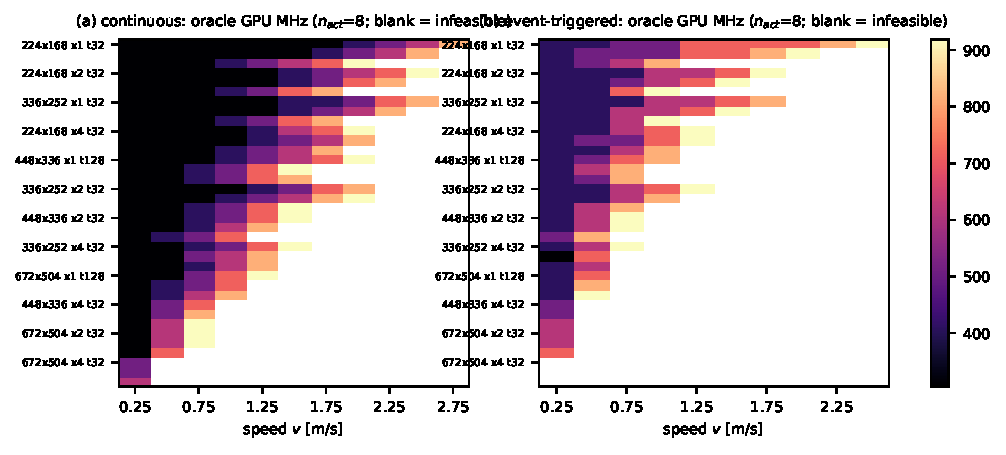
\includegraphics[width=\textwidth]{figs/mot_oracle_gpu.pdf}
  \caption{GPU clock chosen by the offline oracle for each (input, speed) pair ($\nact{=}8$); inputs are
  sorted by $N_{\mathrm{vis}}$. Blank cells are infeasible at every clock.}
  \label{fig:mot-oracle}
\end{figure*}

% =====================================================================================================
\section{Problem Formulation}
\label{sec:problem}

\paragraph{Given}
A task input $x = (\text{resolution}, n_{\mathrm{img}}, N_{\mathrm{txt}}, \nact)$, a speed $v$ set by the
planner, the decision distance $D$, and an invocation mode.
\paragraph{Decision}
A DVFS point $f = (f_{\mathrm{CPU}}, f_{\mathrm{GPU}}) \in \mathcal{F}$.
\paragraph{Objective}
Minimise the average compute power while staying safe:
\begin{align}
  f^\star(x, v) = \arg\min_{f\in\mathcal{F}} \;& \bar P(f; x, v)  \label{eq:obj}\\
  \text{s.t.}\;& \Lq(f; x, \nact) \le B(v). \nonumber
\end{align}
We consider two invocation modes:
\begin{itemize}
  \item \emph{Continuous}: queries run back to back and the VLM stops after $\nact$ tokens, so
        $\bar P = E_{\mathrm{req}}(f;x)/L(f;x)$ and $B(v) = \tau(v)$.
  \item \emph{Event-triggered}: one query every $d_q$ metres, i.e.\ with period $T_q = d_q/v$, and the board idles in between:
        \begin{equation}
          \bar P = \frac{E_{\mathrm{req}}(f;x) + P_{\mathrm{idle}}(f)\,\bigl(T_q - L(f;x)\bigr)}{T_q},
          \quad B(v) = \min\bigl(\tau(v),\, T_q\bigr).
        \end{equation}
\end{itemize}
Here $E_{\mathrm{req}}$ and $L$ are the energy and median latency of a request up to its $\nact$-th token.

\paragraph{Why the speed is given}
Mechanical energy is constant for a given $v$, so leaving it out of \cref{eq:obj} is exact.
If $v$ were also a decision variable, minimising the compute energy of a mission of length $S$,
$\bar P\, S/v$, is solved by the fastest feasible speed at near-maximum clocks for most inputs (86\%
continuous, 97\% event-triggered in our data): the problem degenerates.
The planner instead fixes $v$ from the environment, and $v_{\max}(x) = v^*(\Lq(f_{\max};x))$ is a
capability limit we report to it.
\paragraph{Dual form}
Under a power budget $P_{\mathrm{b}}$, the same data answer
$\max_f v^*(f;x)$ s.t.\ $\bar P(f;x) \le P_{\mathrm{b}}$, i.e.\ the speed–power Pareto front.

% =====================================================================================================
\section{Experimental Setup}
\label{sec:exp}

\paragraph{Platform and workload}
Jetson Orin NX 16\,GB (JetPack R36.4.7); CPU clocks \{576, 1190, 1984\}\,MHz; GPU clocks
\{306, 408, \dots, 918\}\,MHz; board power from the on-board INA3221 sampled every 20\,ms.
Qwen2.5-VL-3B-Instruct (Q4\_K\_M weights, F16 vision projector) runs through llama.cpp's multimodal API.
Each input and DVFS point is measured 5 times after 2 warm-up runs, and idle power is measured for 30\,s at each point.

\paragraph{Scenarios}
A scenario is (mode, $\nact\in\{8,16,32\}$, input, $v \in \{0.25, 0.5, \dots, 3\}$\,m/s), with $d_q{=}\Dq$\,m in
the event-triggered mode. We keep the \NScen{} scenarios in which at least one DVFS point satisfies the
constraint. Policies are evaluated trace-driven: each policy picks a DVFS point per scenario, and its
power and latency are taken from the measurements at that point.

\paragraph{Baselines}
\begin{itemize}
  \item \textbf{MaxPerf}: highest CPU and GPU clocks (1984/918\,MHz).
  \item \textbf{Governor}: stock Jetson governors (schedutil for the CPU, nvhost\_podgov for the GPU).
  \item \textbf{MinCPU-MaxGPU}: lowest CPU and highest GPU clock, a race-to-idle heuristic motivated by O3.
  \item \textbf{Speed-only}: knows $v$ but not the input; it uses one DVFS point per $(\text{mode}, \nact, v)$
        that is feasible for every input, choosing the cheapest such point.
  \item \textbf{Input-only}: knows the input but not $v$; it uses one DVFS point per $(\text{mode}, \nact, x)$
        that is feasible at every speed.
  \item \textbf{Oracle}: solves \cref{eq:obj} per scenario using the measured $\Lq$ and $\bar P$. It is an offline upper
        bound for any policy that knows both the input and the speed.
\end{itemize}
\paragraph{Metrics}
Average power $\bar P$, saving versus MaxPerf, and the deadline-violation rate, i.e.\ the fraction of
measured requests at the chosen point whose $\mathrm{TTA}(\nact)$ exceeds $B(v)$.

% =====================================================================================================
\section{Baseline Results}
\label{sec:exp-results}

\begin{table}[t]
  \centering
  \caption{Baselines averaged over \NScen{} feasible scenarios ($\nact \in \{8,16,32\}$).}
  \label{tab:baselines}
  \scriptsize
  \setlength{\tabcolsep}{3pt}
  \begin{tabular}{lrrrrrr}
\toprule
 & \multicolumn{3}{c}{Continuous} & \multicolumn{3}{c}{Event-triggered ($d_q$=2\,m)} \\
\cmidrule(lr){2-4}\cmidrule(lr){5-7}
Policy & $\bar P$ [W] & Saving [\%] & Viol. [\%] & $\bar P$ [W] & Saving [\%] & Viol. [\%] \\
\midrule
MaxPerf & 15.66 & 0.0 & 0.8 & 11.60 & 0.0 & 0.7 \\
Governor & 13.83 & 11.8 & 8.4 & 10.76 & 7.5 & 12.8 \\
MinCPU-MaxGPU & 13.26 & 15.3 & 0.9 & 10.05 & 13.2 & 1.2 \\
Speed-only & 12.33 & 21.1 & 0.0 & 10.03 & 13.6 & 0.0 \\
Input-only & 12.58 & 19.6 & 0.0 & 9.86 & 14.9 & 0.0 \\
\midrule
Oracle (input+speed) & 9.61 & 38.6 & 0.0 & 9.48 & 18.7 & 0.0 \\
\bottomrule
\end{tabular}

\end{table}

\begin{figure}[t]
  \centering
  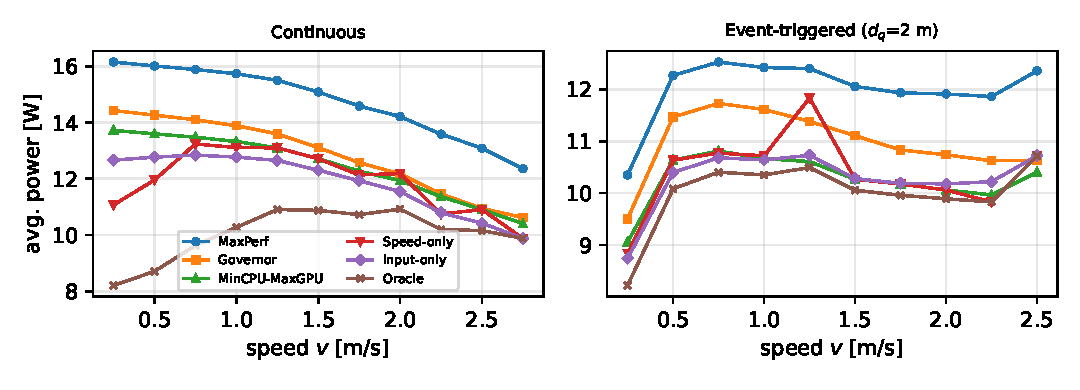
\includegraphics[width=\columnwidth]{figs/baselines_power_vs_speed.pdf}
  \caption{Average power versus speed (mean over feasible inputs and $\nact$).}
  \label{fig:baselines}
\end{figure}

\Cref{tab:baselines} and \cref{fig:baselines} summarise the results.
\begin{itemize}
  \item \emph{Governor}: saves only \GovSaveCont\% (continuous) and \GovSaveEvent\% (event-triggered)
        over MaxPerf, and violates the deadline in \GovViolCont\% and \GovViolEvent\% of requests,
        because it runs below the maximum GPU clock exactly when high speed needs it.
  \item \emph{MinCPU-MaxGPU}: already saves \RaceSaveCont\%/\RaceSaveEvent\%, confirming that the CPU clock
        is wasted power.
  \item \emph{One-dimensional policies}: Speed-only and Input-only save \SpeedOnlySaveCont\% and
        \InputOnlySaveCont\% (continuous), because each must provision for the worst case of the
        dimension it cannot see.
  \item \emph{Oracle}: saves \OracleSaveCont\% (continuous) and \OracleSaveEvent\% (event-triggered) over
        MaxPerf, and \OracleVsGovCont\%/\OracleVsGovEvent\% over the governor.
\end{itemize}
The gap between Oracle and the one-dimensional policies is the headroom for an input- and
speed-aware controller. It is large when the VLM runs continuously, and smaller in the event-triggered
mode, where idle power dominates the average.

\todo{Our method: predict $\Lq(f;x,\nact)$ from the input and solve \cref{eq:obj} online; compare with Oracle.}

\end{document}
